%!TEX program = xelatex
% 完整编译: xelatex -> bibtex -> xelatex -> xelatex
\documentclass[lang=cn,11pt,a4paper,cite=authoryear]{elegantpaper}

\title{实验数据整合}
\author{孙凯威}
\institute{\href{sunkaiwei@cug.edu.cn}{中国地质大学(武汉)}}

\date{\zhtoday}

% 本文档命令
\usepackage{array}
\usepackage{xcolor}
\usepackage{colortbl}
\newcommand{\ccr}[1]{\makecell{{\color{#1}\rule{1cm}{1cm}}}}

\begin{document}

\maketitle

\section{实验一}

\subsection{固定参数}

本实验所固定的参数有各分支的各层激活函数均为$sigmoid$函数,优化器选择使用$Adam$优化器,所设置的学习率$\epsilon$为0.0001,训练的迭代次数$epoach$为800,训练的批大小$mini-batch$ $size$为2048,$DBN$的层数为5层,预训练的批大小$batch-size$为64.

对于空间-光谱分支,我们使用5层$DBN$,隐藏层节点数为1500.对于地形分支我们固定$DBN$层数也为5层,隐藏层节点数需要进行选择。

\subsection{方案一:无全连接层+单输出}
在两个分支进行合并后直接送入$softmax$分类器进行分类,分类的输出方式为单输出,即只输出20个二级地物标签的类别。所需调节的超参数为地形分支的各层的节点数,所选取范围为[3-1500].

每个节点数运行5次,取平均值和去极值平均两种方法。部分节点的五次结果和平均结果如表\ref{tab:addlabel}所示,每个节点的五次平均值可见图\ref{fig:shuju1}
去极值平均的结果可以见图\ref{fig:shuju1qujizhi}.由图可以看出,当地形分支节点数为550时,实验的验证集结果最好,故选定地形分支节点数为550。

% Table generated by Excel2LaTeX from sheet 'Sheet1'
\begin{table}[htbp]
  \centering
  \caption{实验数据表格片段}
    \begin{tabular}{|c|c|c|c|c|c|c|c|}
    \toprule
          & \textbf{300} & \textbf{350} & \textbf{400} & \textbf{450} & \textbf{500} & \textbf{550} & \textbf{600} \\
    \midrule
    \textbf{1} & 0.9048 & 0.9107 & 0.9139 & 0.9083 & 0.8939 & 0.9133 & 0.9107 \\
    \midrule
    \textbf{2} & 0.9083 & 0.9108 & 0.9126 & 0.9098 & 0.9123 & 0.9107 & 0.8974 \\
    \midrule
    \textbf{3} & 0.9008 & 0.9104 & 0.9097 & 0.9167 & 0.9077 & 0.908 & 0.8717 \\
    \midrule
    \textbf{4} & 0.8995 & 0.9136 & 0.8996 & 0.9112 & 0.9148 & 0.9136 & 0.8959 \\
    \midrule
    \textbf{5} & 0.907 & 0.9034 & 0.9119 & 0.911 & 0.9128 & 0.9124 & 0.9113 \\
    \midrule
    平均    & 0.90408 & \cellcolor[rgb]{ 1,  .6,  .8}0.90978 & 0.90954 & \cellcolor[rgb]{ 1,  0,  0}0.9114 & 0.9083 & \cellcolor[rgb]{ .753,  0,  0}0.9116 & 0.8974 \\
    \midrule
    去极值平均 & 0.9042 & 0.910633 & \cellcolor[rgb]{ 1,  0,  0}0.9114 & 0.910667 & \cellcolor[rgb]{ 1,  .6,  .8}0.910933 & \cellcolor[rgb]{ .753,  0,  0}0.912133 & 0.901333 \\
    \bottomrule
    \end{tabular}%
  \label{tab:addlabel}%
\end{table}%

\begin{figure}[!htb]
  \centering
  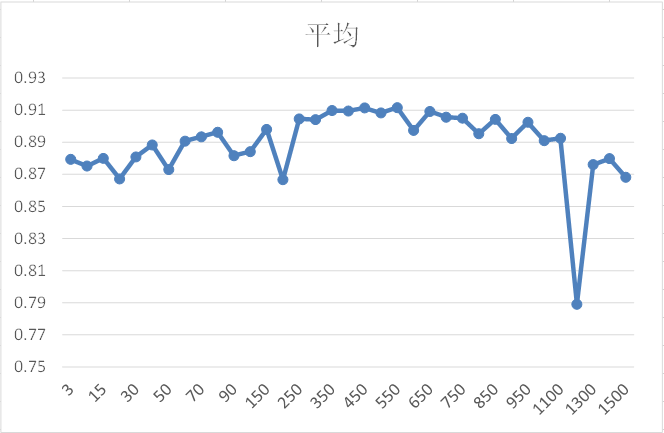
\includegraphics[width=0.9\textwidth]{实验数据1.png}
  \caption{实验数据的平均值}
  \label{fig:shuju1}
\end{figure}

\begin{figure}[!htb]
  \centering
  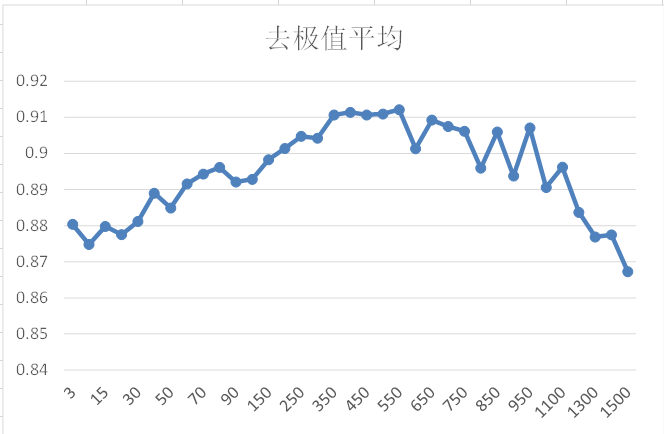
\includegraphics[width=0.9\textwidth]{实验数据1-去极值.png}
  \caption{实验数据的去极值平均值}
  \label{fig:shuju1qujizhi}
\end{figure}

我使用地形分支节点数为550训练出来的模型在测试集上进行预测,并获取了训练集和验证集的正确率和损失值随着迭代次数变化的图,如图\ref{fig:train-acc1}和\ref{fig:train-loss1}
\begin{figure}[!htb]
  \centering
  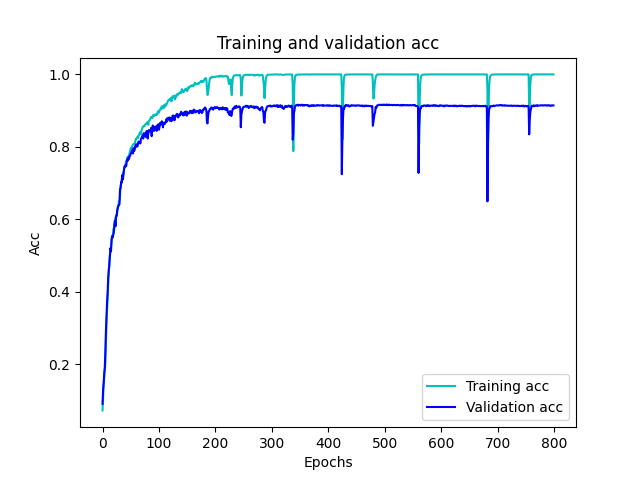
\includegraphics[width=0.9\textwidth]{save_acc2.png}
  \caption{地形分支节点数为550的训练集和验证集的实验精度}
  \label{fig:train-acc1}
\end{figure}
\begin{figure}[!htb]
  \centering
  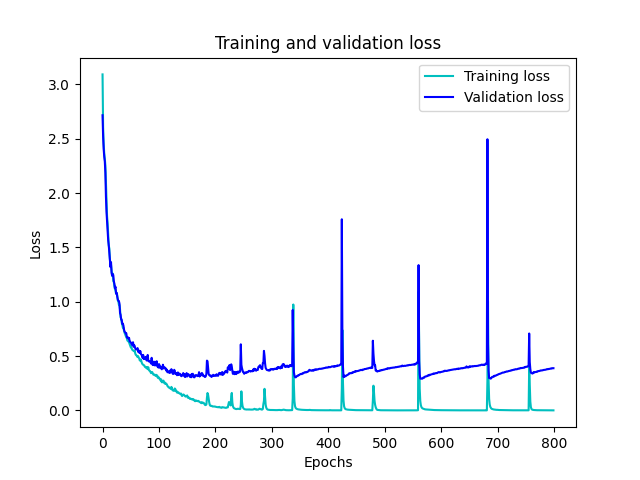
\includegraphics[width=0.9\textwidth]{save_loss2.png}
  \caption{地形分支节点数为550的训练集和验证集的损失值}
  \label{fig:train-loss1}
\end{figure}


\subsection{方案二:无全连接层+多输出}
在两个分支进行合并后直接送入$softmax$分类器进行分类,分类的输出方式为多输出。即输出7个一级地物标签和20个二级地物标签。本实验二的地形分支的节点数选取
方法一中所得到的550.本实验需要调节的超参数为一级地物标签的损失值和二级地物标签的损失值的加权系数。二级地物的系数固定为1,一级地物的系数的所选取的范围为0-1(一步为0.1)和1-10(一步为1)。

每个加权系数运行5次,最后取平均值和去极值平均值。部分加权系数的5次运行所得到的验证集结果如表\ref{tab:table2}所示。
各个加权系数5次运行的正确率平均值可见图\ref{fig:shiyanshu2junzhi},去极值平均的结果可见图\ref{fig:shiyanshu2qujizhi}.
由图\ref{fig:shiyanshu2junzhi}和\ref{fig:shiyanshu2qujizhi}可知,一级地物标签的加权系数为0.3时,实验的验证集正确率最高,故选定一级地物标签的损失值加权系数为0.3.

% Table generated by Excel2LaTeX from sheet 'Sheet1'
\begin{table}[htbp]
  \centering
  \caption{部分加权系数的5次运行结果}
    \begin{tabular}{|c|c|c|c|c|c|}
    \toprule
          & \textbf{0.1} & \textbf{0.2} & \textbf{0.3} & \textbf{0.4} & \textbf{0.5} \\
    \midrule
    \textbf{1} & 0.911 & 0.9023 & 0.9113 & 0.91  & 0.8985 \\
    \midrule
    \textbf{2} & 0.9113 & 0.9138 & 0.9135 & 0.9058 & 0.9111 \\
    \midrule
    \textbf{3} & 0.9113 & 0.9087 & 0.9118 & 0.916 & 0.9077 \\
    \midrule
    \textbf{4} & 0.9131 & 0.9136 & 0.9125 & 0.8999 & 0.8815 \\
    \midrule
    \textbf{5} & 0.9131 & 0.9112 & 0.914 & 0.914 & 0.9124 \\
    \midrule
    平均    & \cellcolor[rgb]{ 1,  0,  0}0.91196 & 0.90992 & \cellcolor[rgb]{ .753,  0,  0}0.91262 & 0.90914 & 0.90224 \\
    \midrule
    去极值平均 & \cellcolor[rgb]{ 1,  0,  0}0.9119 & 0.911167 & \cellcolor[rgb]{ .753,  0,  0}0.9126 & 0.909933 & 0.905767 \\
    \bottomrule
    \end{tabular}%
  \label{tab:table2}%
\end{table}%

\begin{figure}[!htb]
  \centering
  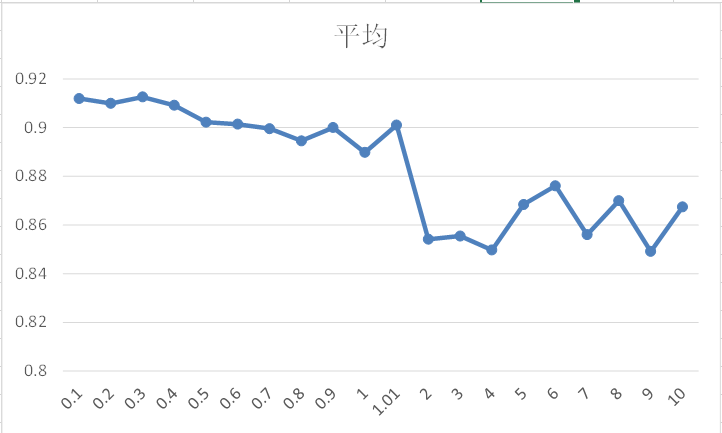
\includegraphics[width=0.9\textwidth]{实验数据2-均值.png}
  \caption{各个加权系数5次运行的正确率平均值}
  \label{fig:shiyanshu2junzhi}
\end{figure}

\begin{figure}[!htb]
  \centering
  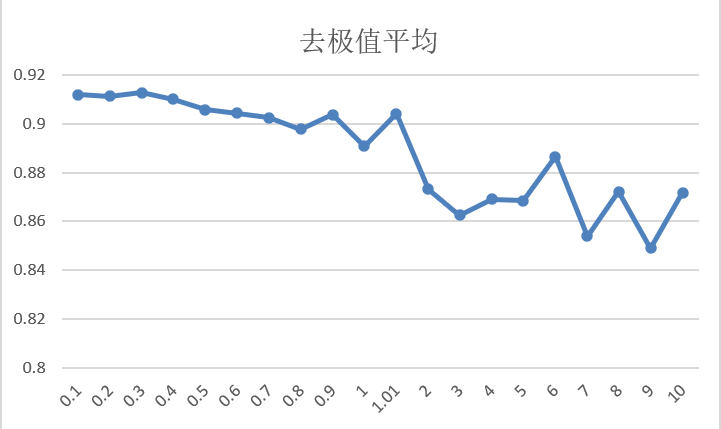
\includegraphics[width=0.9\textwidth]{图片1.png}
  \caption{各个加权系数5次运行的正确率去极值平均值}
  \label{fig:shiyanshu2qujizhi}
\end{figure}

我使用一级地物加权系数为0.3训练得到的模型对测试集进行预测,并获取了其在训练集和验证集上的正确率和损失值随着迭代次数变化的图,其中验证集的变化如图\ref{fig:val-acc2}和\ref{fig:val-loss2}所示

\begin{figure}[!htb]
  \centering
  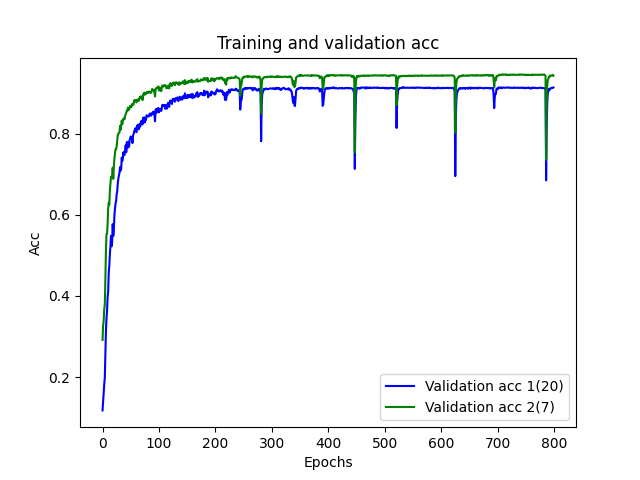
\includegraphics[width=0.9\textwidth]{save_Va_acc-1-3.0.png}
  \caption{一级地物的加权系数为0.3的验证集正确率}
  \label{fig:val-acc2}
\end{figure}

\begin{figure}[!htb]
  \centering
  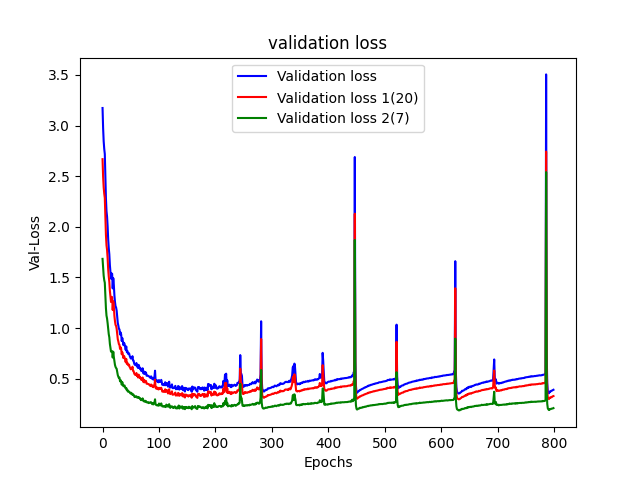
\includegraphics[width=0.9\textwidth]{save_Va_loss-1-3.0.png}
  \caption{一级地物的加权系数为0.3的验证集损失值}
  \label{fig:val-loss2}
\end{figure}


\subsection{方案三:一个全连接层+单输出}
本实验在两个分支进行合并后再输入到一层全连接层,然后再送入$softmax$分类器进行分类,分类的输出方式为单输出,即只输出20个二级地物标签的类别。本实验没有需要调节的超参数,地形分支节点数为方法一中所选取的550。
全连接层的节点数为空间-光谱分支的节点数与地形分支的节点数的加和,即$1500+550=2050$.

使用该模型对测试集结果进行预测,并获取到其在训练集与验证集上的精度与损失值随着迭代次数的变化情况的图,如图\ref{fig:train-acc3}和\ref{fig:train-loss3}所示。

\begin{figure}[!htb]
  \centering
  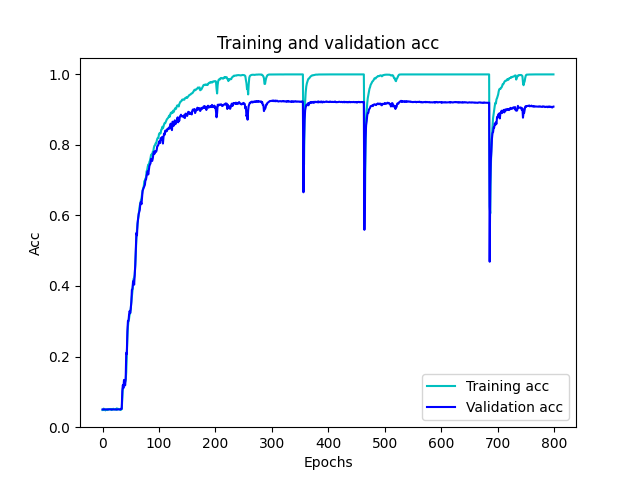
\includegraphics[width=0.9\textwidth]{save_acc3.png}
  \caption{方法三在训练集与验证集上的精度变化}
  \label{fig:train-acc3}
\end{figure}

\begin{figure}[!htb]
  \centering
  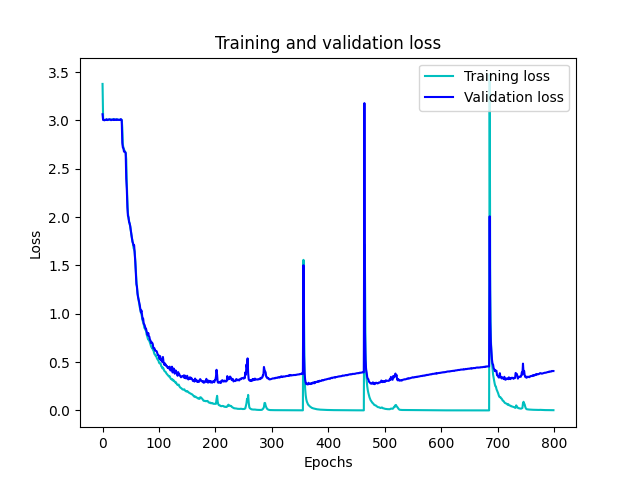
\includegraphics[width=0.9\textwidth]{save_loss3.png}
  \caption{方法三在训练集与验证集上的损失值变化}
  \label{fig:train-loss3}
\end{figure}

\subsection{方法四:一个全连接层+多输出}
本实验在两个分支进行合并后再输入到一层全连接层,然后再送入$softmax$分类器进行分类,分类的输出方式为多输出,即输出7个一级地物标签和20个二级地物标签。本实验四的地形分支的节点数为方法一中所选取的550,一级地物的损失加权系数为方法二中所选取的0.3.全连接层的节点数为空间-光谱分支的节点数与地形分支的节点数的加和,即$1500+550=2050$.

使用该模型对测试集结果进行预测,并获取到其在训练集与验证集上的精度与损失值随着迭代次数的变化情况的图,验证集精度和损失变化如图\ref{fig:val-acc4}和\ref{fig:val-loss4}所示。

\begin{figure}[!htb]
  \centering
  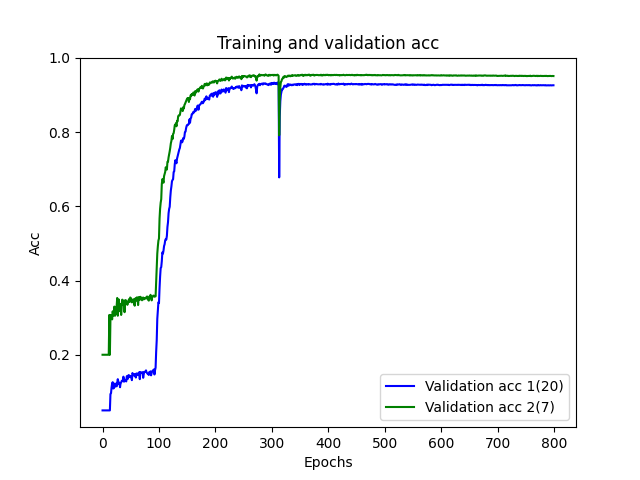
\includegraphics[width=0.9\textwidth]{save_Va_acc-5-3.0.png}
  \caption{方法四在验证集上的精度变化}
  \label{fig:val-acc4}
\end{figure}

\begin{figure}[!htb]
  \centering
  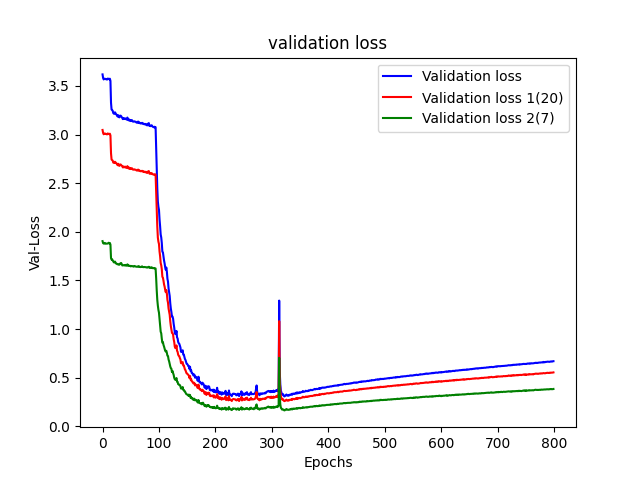
\includegraphics[width=0.9\textwidth]{save_Va_loss-5-3.0.png}
  \caption{方法四在验证集上的损失值变化}
  \label{fig:val-loss4}
\end{figure}


\subsection{方法对比}




\section{协作人员招募}
招募 Elegant\LaTeX{} 的协作人员,没有工资。工作内容:翻译 Elegant\LaTeX{} 系列模板相关的文稿(中翻英),维护模板的 wiki(主要涉及 Markdown),如果有公众号文稿写作经历的话,也可以帮忙写微信稿。本公告长期有效。

目前 ElegantLaTeX 共有 4 名协作人员,分别是
\begin{itemize}
  \item 官方文档翻译: \href{https://github.com/peggy2006xzyz}{YPY};
  \item GitHub 维基维护: \href{https://github.com/izinngo}{Ingo Zinngo}、\href{https://github.com/xiaohao890809}{追寻原风景};
  \item QQ 群管理员: \href{https://github.com/sikouhjw}{Sikouhjw}.
\end{itemize}

在此感谢他们无私的奉献!


\section{致谢}
截止到 2020 年 04 月 12 日,ElegantPaper v0.09 版本发布,ElegantPaper 模板在 GitHub 上的收藏数(star)达到了 277。在此特别感谢 China\TeX{} 以及 \href{http://www.latexstudio.net/}{\LaTeX{} 工作室}对于本系列模板的大力宣传与推广。如果你喜欢我们的模板,你可以在 GitHub 上收藏(Star)我们的模板。
\begin{figure}[htbp]
  \centering
  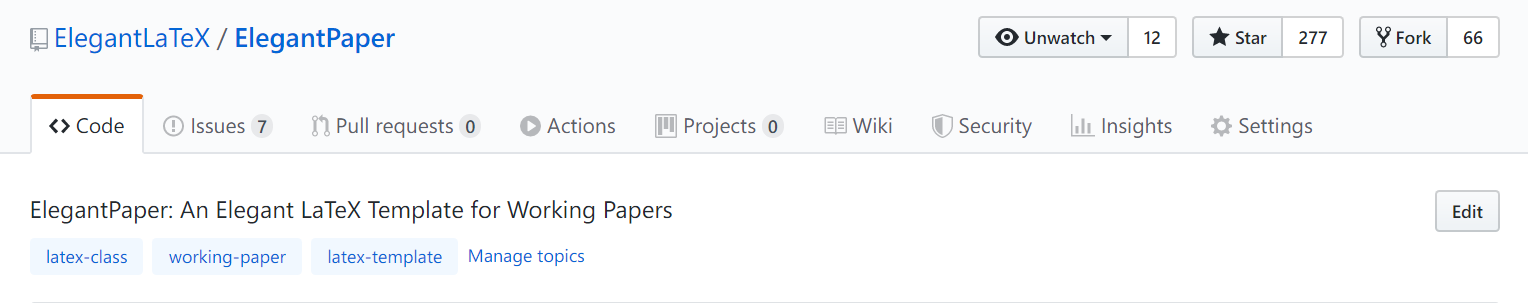
\includegraphics[width=\textwidth]{star.png}
  \caption{一键三连求赞}
\end{figure}

\section{捐赠}
如果您非常喜爱我们的模板,你还可以选择捐赠以表达您对我们模板和我的支持!

\begin{figure}[htbp]
  \centering
  
\includegraphics[width=0.5\textwidth]{donate.jpg}
\end{figure}

\textbf{赞赏费用的使用解释权归 Elegant\LaTeX{} 所有,并且不接受监督,请自愿理性打赏}。10 元以上的赞赏,我们将列入捐赠榜,谢谢各位金主!


\begin{table}[!htb]
  \centering
  \caption{Elegant\LaTeX{} 系列模板捐赠榜}
    \begin{tabular}{*{4}{>{\scriptsize}c}|*{4}{>{\scriptsize}c}}
    \hline
    \textbf{捐赠者} & \textbf{金额} & \textbf{时间} & \textbf{渠道} & \textbf{捐赠者} & \textbf{金额} & \textbf{时间} & \textbf{渠道} \\
    \hline
    Lerh  & 10 RMB & 2019/05/15 & 微信    & 越过地平线 & 10 RMB & 2019/05/15 & 微信 \\
    银桑    & 20 RMB & 2019/05/27 & 微信    & *空    & 10 RMB & 2019/05/30 & 微信 \\
    latexstudio.net & 666 RMB & 2019/06/05 & 支付宝   & A*n   & 40 RMB & 2019/06/15 & 微信 \\
    * 夏   & 22 RMB & 2019/06/15 & 微信    & * 倩   & 21 RMB  & 2019/06/15 & 微信 \\
    Cassis & 11 RMB & 2019/06/30 & 微信    & *君    & 10 RMB & 2019/07/23 & 微信 \\
    P*u   & 50 RMB & 2019/07/30 & 微信    & *萌    & 19 RMB & 2019/08/28 & 微信 \\
    曲豆豆   & 10 RMB & 2019/08/28 & 微信    & 李博    & 100 RMB & 2019/10/06 & 微信 \\
    Njustsll & 10 RMB & 2019/10/11 & 微信    & 刘志阔   & 99.99 RMB & 2019/10/15 & 支付宝 \\
    * 韬   & 16 RMB & 2019/10/17 & 微信    & 赤霓    & 12 RMB & 2019/10/17 & 支付宝 \\
    追寻原风景 & 10 RMB & 2019/10/28 & 微信    & 郭德良   & 88 RMB & 2019/11/03 & 微信 \\
    自强不息  & 20 RMB & 2019/11/04 & 支付宝   & 读书之虫  & 20 RMB & 2019/11/18 & 微信 \\
    *等    & 10 RMB & 2019/11/18 & 微信    & *哲    & 20 RMB & 2019/11/18 & 微信 \\
    佚名    & 10 RMB & 2019/11/24 & 微信    & Jiye Qian & 66 RMB & 2019/12/04 & 微信 \\
    * 阳   & 20 RMB & 2019/12/05 & 微信    & Catcher & 11 RMB & 2019/12/08 & 支付宝 \\
    希尔波特门徒 & 10 RMB & 2019/12/09 & 支付宝   & * 伟   & 10 RMB & 2019/12/09 & 微信 \\
    Simon & 20 RMB & 2019/12/11 & 支付宝   & 流殇丶浅忆 & 66.60 RMB & 2019/12/18 & 支付宝 \\
    羽     & 10 RMB & 2019/12/20 & 支付宝   & * 琛   & 15 RMB & 2019/12/20 & 微信 \\
    随风    & 20 RMB & 2019/12/27 & 支付宝   & Ws    & 23.30 RMB & 2019/12/28 & 微信 \\
    初八    & 100 RMB  & 2020/01/02 & 支付宝   & p*e   & 20 RMB & 2020/01/03 & 微信 \\
    Shunmx & 100 RMB & 2020/01/03 & 微信    & hj    & 10 RMB & 2020/01/03 & 微信 \\
    F*5   & 10 RMB & 2020/01/03 & 微信    & S*m   & 20.20 RMB & 2020/01/03 & 微信 \\
    二代青雉  & 13 RMB & 2020/01/14 & 支付宝   & *?    & 66 RMB & 2020/01/15 & 微信 \\
    Mr. Xiong & 20 RMB & 2020/01/17 & 微信    & *博    & 15 RMB & 2020/01/18 & 微信 \\
    * 者  & 10 RMB & 2020/02/02 & 微信    & Jackie  &  88.80 RMB  &  2020/02/09 & 微信 \\
    Henry\_Sun、 & 50 RMB & 2020/02/14 & 支付宝 & * 桥  & 50 RMB & 2020/02/21 & 微信 \\
    昀琏 & 10 RMB & 2020/03/02 & 支付宝 & S*y  &  10 RMB  &  2020/03/15 & 微信 \\
    * 哥  & 66.66 RMB & 2020/03/17 & 微信    &   K*e & 30 RMB & 2020/03/30 & 微信\\
    * 阳  &  20 RMB  &  2020/04/02 & 微信 & 士*n  & 30 RMB & 2020/04/11 & 微信 \\
    \hline
    \end{tabular}%
  \label{tab:donation}%
\end{table}%

\section{常见问题 FAQ}

\begin{enumerate}[label=\arabic*).]
  \item \textit{如何删除版本信息?}\\
      导言区不写 \lstinline|\version{x.xx}| 即可。
  \item \textit{如何删除日期?}\\
      需要注意的是,与版本 \lstinline{\version} 不同的是,导言区不写或注释 \lstinline{\date} 的话,仍然会打印出当日日期,原因是 \lstinline{\date} 有默认参数。如果不需要日期的话,日期可以留空即可,也即 \lstinline|\date{}|。
  \item \textit{如何获得中文日期?}\\
      为了获得中文日期,必须在中文模式下\footnote{英文模式下,由于未加载中文宏包,无法输入中文。},使用 \lstinline|\date{\zhdate{2019/10/11}}|,如果需要当天的汉化日期,可以使用 \lstinline|\date{\zhtoday}|,这两个命令都来源于 \href{https://ctan.org/pkg/zhnumber}{\lstinline{zhnumber}} 宏包。
  \item \textit{如何添加多个作者?}\\
      在 \lstinline{\author} 里面使用 \lstinline{\and},作者单位可以用 \lstinline{\\} 换行。\begin{lstlisting}
\author{author 1\\ org. 1 \and author 2 \\ org. 2 }
\end{lstlisting}
  \item \textit{如何添加中英文摘要?}\\
      请参考 \href{https://github.com/ElegantLaTeX/ElegantPaper/issues/5}{GitHub::ElegantPaper/issues/5}
\end{enumerate}

\section{示例}

为了让大家更加清楚最终的论文效果,如下给出两篇使用 ElegantPaper 模板排版的工作论文示例,也欢迎大家“投稿”!

\begin{enumerate}
  \item \href{https://github.com/EthanDeng/bank-custody}{银行存管、投资者决策与 P2P 网络借贷规范发展};
  \item \href{https://github.com/EthanDeng/risk-awareness}{互联网金融风险与投资者风险意识 —— 来自网贷平台交易数据的证据}。
\end{enumerate}


\nocite{*}
\bibliography{wpref}

\appendix
%\appendixpage
\addappheadtotoc
\section{使用 newtx 系列字体}

如果需要使用原先版本的 \lstinline{newtx} 系列字体,可以通过显示声明数学字体:

\begin{lstlisting}
\documentclass[math=newtx]{elegantbook}
\end{lstlisting}

\subsection{连字符}

如果使用 \lstinline{newtx} 系列字体宏包,需要注意下连字符的问题。
\begin{equation}
  \int_{R^q} f(x,y) dy.\emph{of\kern0pt f}
\end{equation}
的代码为
\begin{lstlisting}
\begin{equation}
  \int_{R^q} f(x,y) dy.\emph{of \kern0pt f}
\end{equation}
\end{lstlisting}

\subsection{宏包冲突}

另外在 ElegantBook 模板中,有用户反馈模板在使用 \lstinline{yhmath} 以及 \lstinline{esvect} 等宏包时会报错:
\begin{lstlisting}
LaTeX Error:
   Too many symbol fonts declared.
\end{lstlisting}

原因是在使用 \lstinline{newtxmath} 宏包时,重新定义了数学字体用于大型操作符,达到了 {\heiti 最多 16 个数学字体} 的上限,在调用其他宏包的时候,无法新增数学字体。为了减少调用非常用宏包,在此给出如何调用 \lstinline{yhmath} 以及 \lstinline{esvect} 宏包的方法。

请在 \lstinline{elegantpaper.cls} 内搜索 \lstinline{yhmath} 或者 \lstinline{esvect},将你所需要的宏包加载语句\textit{取消注释}即可。
\begin{lstlisting}
%%% use yhmath pkg, uncomment following code
% \let\oldwidering\widering
% \let\widering\undefined
% \RequirePackage{yhmath}
% \let\widering\oldwidering

%%% use esvect pkg, uncomment following code
% \RequirePackage{esvect}
\end{lstlisting}


\end{document}
